% TeX file "application"

% Research Module in Econometrics & Statistics 
% Prof. Dr. Liebl & Dr. Christopher Walsh
% Winter 2021/22, M.Sc. Economics, Bonn University
% Xingyu Tao, Xuan Li, Sven Jacobs


\section{Application} \label{sec:application}

To showcase the practical use of the boundary correction methods,
we consider the nonparametric estimation of treatment effects in the regression discontinuity design (RDD).
RDD is a popular quasi-experimental research design to identify a causal effect as a jump of an outcome variable
at a known threshold of a so-called assignment variable.
This threshold constitutes a boundary.
When measuring the size of the discontinuity, i.e.\ the causal effect in a valid RDD,
boundary effects may severely bias the estimate and inference.
RDD was first applied by \textcite{Thistlethwaite_1960}.
\textcite{Hahn_2001} were the first to suggest local linear regression to estimate the conditional expectation function
at the threshold to avoid boundary bias.
Also see \textcite{Porter_2003}.
\textcite{Imbens_2012} investigated bandwidth choice specifically for RDD. 

In a widely-cited study \textcite{Lee_2008} applied RDD to analyze the causal effect of party incumbency on reelection probabilities in U.S. House elections.
Figure~\ref{fig:application_overview} shows the Democrats' probability of winning a seat in the U.S. House of Representatives in the next election against the Democratic vote share minus the vote share of the strongest opponent (almost always the Republicans).
Each data point is an average of the indicator variable for winning election $t+1$ for each interval, which is 0.005 wide.
To the left of the zero-threshold the Democratic nominee lost election t;
to the right, the Democratic party won.
We can see a smooth relationship between the two variables (higher reelection probability for a higher vote share),
except for the threshold at zero which decides about victory or defeat.
\textcite{Lee_2008} interprets the large discontinuity as the true electoral incumbency advantage
as he argues that due to the inherent uncertainty in the exact vote share, winning a close election is \enquote{as good as random}.
Then, districts where the Democrats just barely lost constitute a valid counterfactual for districts where the Democrats just barely won and became incumbent (receiving treatment).

The task is now to estimate the size of the discontinuity.
Figure~\ref{fig:application_fits} displays the fit of each method (NW, LL regression, boundary-adjusted NW) for each side of the threshold.
To select the bandwidths (we allow the degree of smoothing to differ for each side) we use leave-one-out cross-validation (LOOCV).
That is, the bandwidth that minimizes the sum of squared prediction errors:
\begin{align}
	h_{\text{\tiny CV}} &\equiv \argmin_{h \,>\, 0} \CV(h) \,, \text{where} \\
	\CV(h) &\equiv \frac{1}{n} \sum_{i = 1}^{n} (Y_i - \hat{m}_{-i}(X_i, h))^2 \equiv \frac{1}{n} \sum_{i = 1}^{n} \tilde{\epsilon}_i^2 \,.
\end{align}  
One can show that $h_{\text{\tiny CV}}$ is essentially an unbiased estimator of $h_{\text{\tiny MISE}}$ \parencite[Theorem~19.7]{Hansen_2022}.
The solution has to be obtained numerically, which can cause problems.
The function $\CV(h)$ can have multiple local minima (Figures~\ref{fig:application_left_nw}, \ref{fig:application_right_ll})
and the solution can be unbounded such that $h_{\text{\tiny CV}} = \infty$ (Figure~\ref{fig:application_left_ll}).
From the Figures~\ref{fig:application_left} and \ref{fig:application_right} we see that the cross-validated bandwidths are larger for the left side and for the LL estimator.  

\begin{figure}
	\centering
	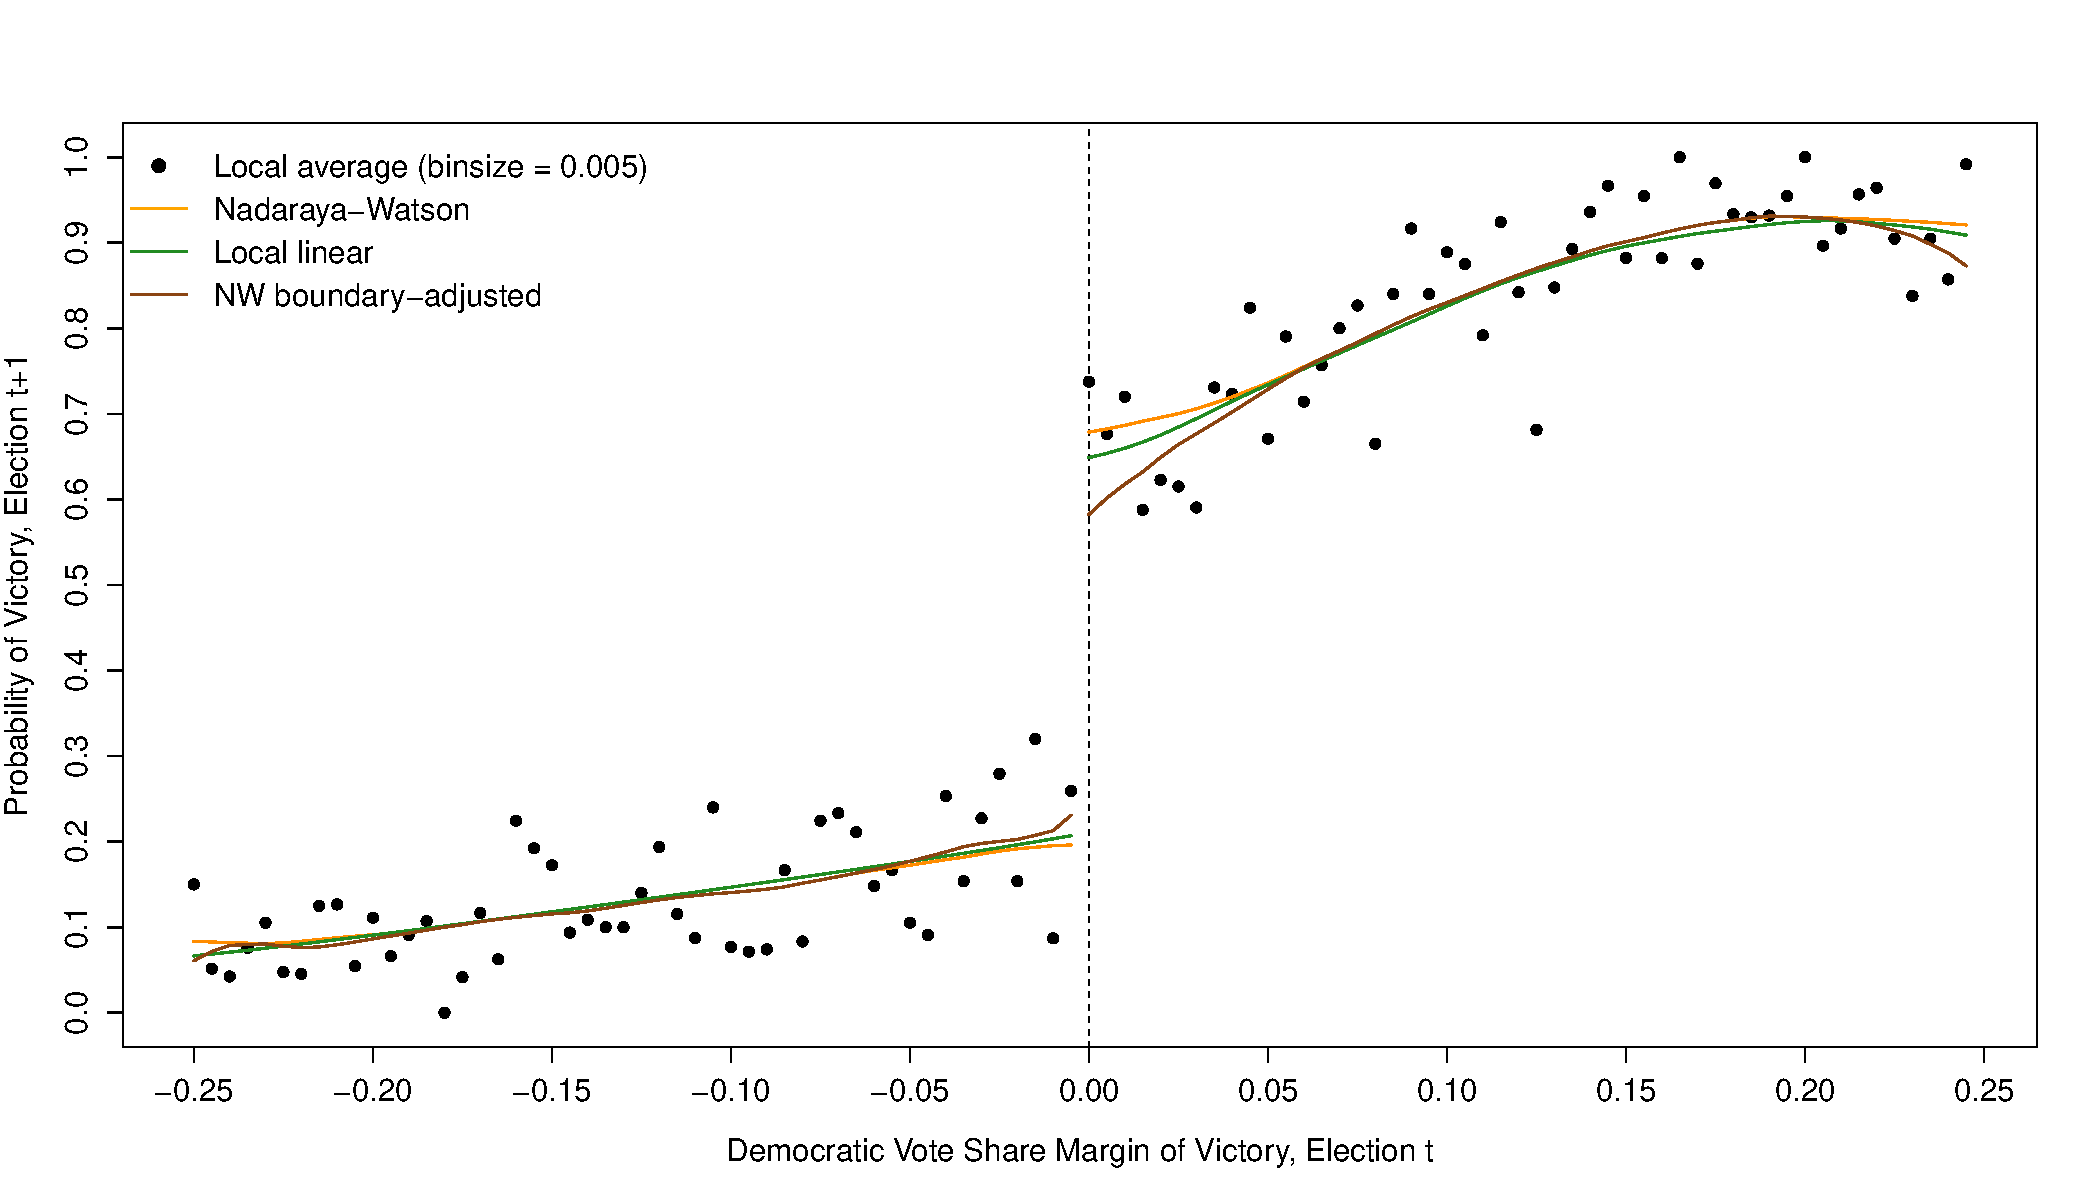
\includegraphics[trim=0 15 20 50, clip, width=0.75\textwidth]{figure_05.pdf}
	\caption{Democrats' probability of victory in election $t+1$, by margin of victory in election $t$.
			 Estimates of NW, LL regression and adjusted NW with cross-validated bandwidths.}
	\label{fig:application_fits}
\end{figure}

The estimates to the left side of the threshold look very similar.
However, since LL regression coincides with the global OLS fit (infinite bandwidth) the estimate is more stable yet captures the same structure.
In contrast, on the right side the estimates differ considerably near the boundary.
It is apparent that the NW estimate suffers from boundary bias as described in Section~\ref{sec:local_linear_regression}.
The explicit boundary adjustment results in a much smaller boundary estimate.
The curve resembles the parametric logit fit of \textcite[Fig.\ 5a]{Lee_2008}.
LL regression also leads to a smaller discontinuity estimate, but the correction is less strong.
Besides, the estimate is less wavy.
The figure illustrates the need for boundary correction.
Just looking at the right side to the threshold, NW suggests a ten percentage points greater incumbency advantage compared to adjusted NW;
and a more than three percentage points greater advantage compared to the LL estimator.
Based on Figure~\ref{fig:application_fits}, the simulation results and its simplicity we pick the LL estimator for further discussion.

We can construct asymptotic confidence intervals to assess precision.
Theorem~\ref{theorem_5} states that the local polynomial estimator is asymptotically normal with a nonparametric $\sqrt{nh}$-rate of convergence and a non-zero bias term.
\begin{theorem} \label{theorem_5}
	Let assumptions \ref{A1}--\ref{A5} be fulfilled and $\E [ \epsilon^{2 + \delta} \,|\, X = x ] < \infty$ for some $\delta > 0$.
	Then, for the local polynomial estimator $\hat{m}$ it holds that
	\begin{align}
		\sqrt{nh} \left( \hat{m}(x) - m(x) - \Bias(\hat{m}(x) \,|\, \bm{X}) \right) &\overset{d}{\longrightarrow} \mathcal{N} \left( 0, \frac{R(K) \sigma^2(x)}{f(x)} \right) \,, \\
		\frac{\hat{m}(x) - \E[\hat{m}(x) \,|\, \bm{X}]}{\sqrt{\Var(\hat{m}(x) \,|\, \bm{X})}} &\overset{d}{\longrightarrow} \mathcal{N}(0, 1) \,.
	\end{align}
\end{theorem}
The proof builds on the CLT, which requires the additional technical moment condition.
See \textcite[Section 19.13]{Hansen_2022}.
An asymptotically valid 95\% confidence interval for $\E[\hat{m}_{\LL}(x) \,|\, \bm{X}]$ is then given by
\begin{equation}
	\hat{m}_{\LL}(x) \pm 1.96 \, \sqrt{\widehat{\Var}(\hat{m}_{\LL}(x) \,|\, \bm{X})} \,, \label{eq:confidence_interval}  
\end{equation}
where with the notation from Section~\ref{subsec:definition}
\begin{equation}
	\widehat{\Var}(\hat{m}_{\LL}(x) \,|\, \bm{X}) = \bm{e}_1^\top \left( \bm{X}_x^\top \bm{W}_x^{\vphantom{\top}} \bm{X}_x^{\vphantom{\top}} \right)^{-1} \bm{X}_x^\top \bm{W}_x^{\vphantom{\top}} \bm{E} \bm{W}_x^{\vphantom{\top}} \bm{X}_x^{\vphantom{\top}} \left( \bm{X}_x^\top \bm{W}_x^{\vphantom{\top}} \bm{X}_x^{\vphantom{\top}} \right)^{-1} \,,
\end{equation}
with $\bm{E} = \diag \{ \tilde{\epsilon}_1^2, \dots, \tilde{\epsilon}_n^2 \}$ as a matrix of the squared prediction errors.
Notice that this interval is not valid for $m(x)$ because bias is not taken into account.%
\footnote{For work on bias-corrected confidence intervals see
		  \citeauthor{Calonico_2018} (\citeyear{Calonico_2018}, \citeyear{Calonico_2022}), \textcite{Cheng_2019}.} 

Figure~\ref{fig:application_confidence_bands} displays the LL estimate along with 95\% approximate confidence bands according to \eqref{eq:confidence_interval}.
We can see that there is more imprecision in the estimator near the threshold.

\begin{figure}
	\centering
	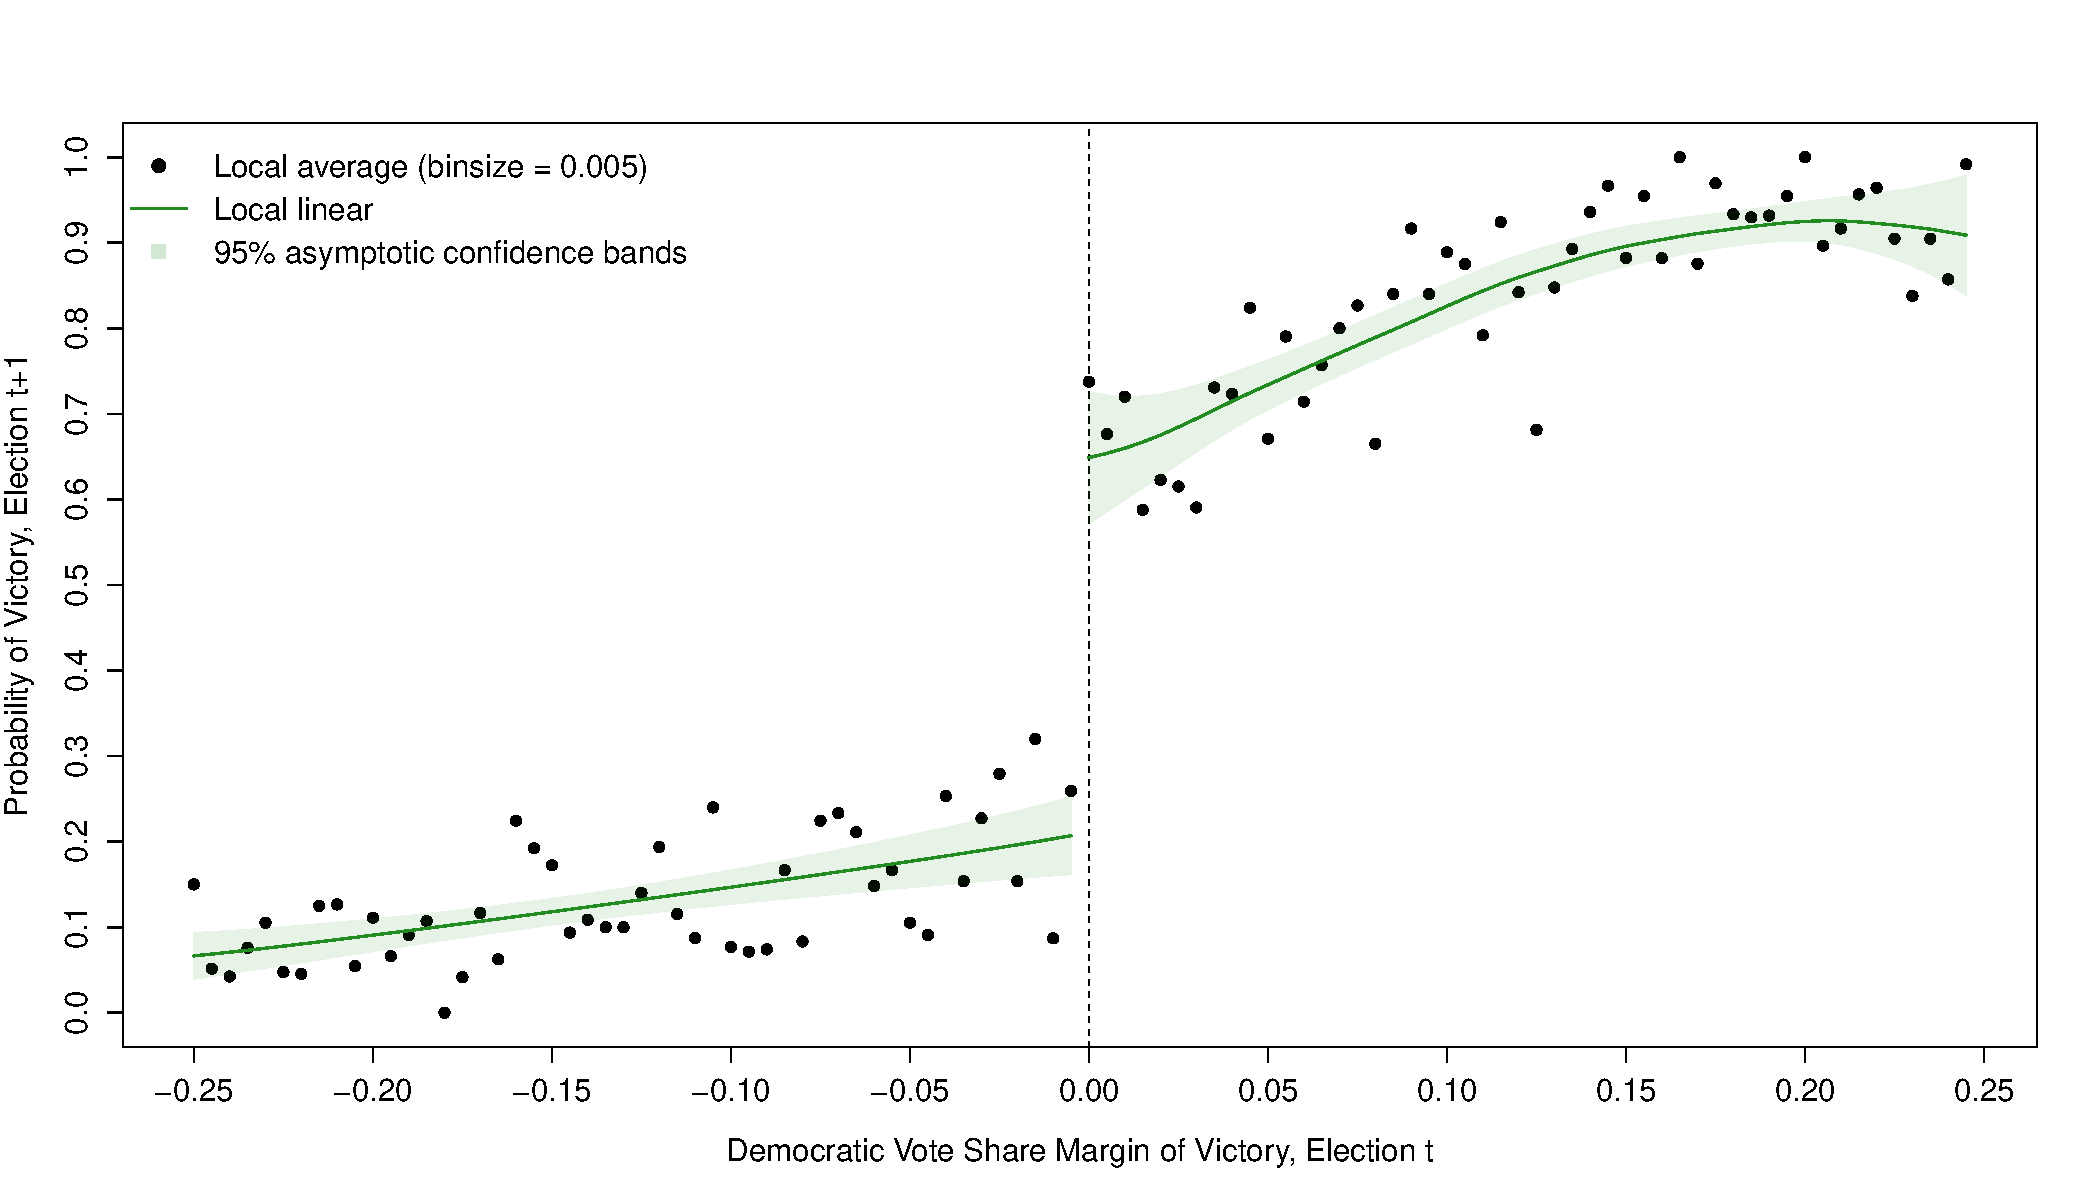
\includegraphics[trim=0 15 20 50, clip, width=0.75\textwidth]{figure_06.pdf}
	\caption{Democrats' probability of victory in election $t+1$, by margin of victory in election $t$.
			 LL estimate along with 95\% approximate confidence bands.}
	\label{fig:application_confidence_bands}
\end{figure}